\documentclass[11pt]{article}
\usepackage[margin=1in]{geometry}
\usepackage{amsmath,amssymb}
\usepackage{booktabs}
\usepackage{array}
\usepackage{enumitem}
\usepackage{parskip}
\usepackage{caption}
\usepackage{subcaption}
\usepackage{tikz}
\usepackage{pgfplots}
\pgfplotsset{compat=1.18}
\usetikzlibrary{positioning,arrows.meta,calc,decorations.pathreplacing}
\setlist{nosep,leftmargin=*}
\captionsetup{font=small}

% vertex colors used in the figures
\definecolor{cY}{HTML}{E8E83A}
\definecolor{cB}{HTML}{2E5BFF}
\definecolor{cR}{HTML}{E23B3B}
\definecolor{cG}{HTML}{3CC83C}
\tikzset{
  v/.style={circle,draw=black!70,inner sep=0pt,minimum size=11pt,font=\scriptsize},
  Y/.style={v,fill=cY}, B/.style={v,fill=cB,text=white},
  R/.style={v,fill=cR,text=white}, G/.style={v,fill=cG},
  W/.style={v,fill=white},
  e/.style={draw=black!55,line width=0.7pt},
  hot/.style={draw=black,line width=1.8pt},
  box/.style={draw,rounded corners=2pt,align=center,font=\small,inner sep=4pt},
  arr/.style={-{Stealth[length=5pt]},line width=0.7pt},
}

\begin{document}

\title{Equitable Graph Coloring:\\ Exact Algorithms for Balanced $k$-Colorings}
\author{Raaj Banga}
\date{November 2026}
\maketitle

%=====================================================================
\section{Problem Statement}\label{sec:problem}

We get a graph and a number of colors $k$. We must color every vertex so
that \textbf{no two neighbors share a color}, using \textbf{all $k$
colors}, and we want the color groups to be \textbf{as close in size as
possible}.

\begin{figure}[h]
\centering
\newcommand{\gone}[7]{%
\begin{tikzpicture}[scale=0.62]
  \node[#1] (1) at (1,1)  {1}; \node[#2] (2) at (2,1)  {2};
  \node[#3] (3) at (0,0)  {3}; \node[#4] (4) at (3,0)  {4};
  \node[#5] (5) at (1,-1) {5}; \node[#6] (6) at (2,-1) {6};
  \foreach \a/\b in {1/2,1/3,2/3,2/4,3/5,3/6,4/6,5/6} \draw[e] (\a)--(\b);
  \node[font=\small,align=center] at (1.5,-2.1) {#7};
\end{tikzpicture}}
\gone{Y}{B}{R}{R}{Y}{B}{group sizes $(2,2,2)$\\score $0$ \checkmark{} best}\qquad\qquad
\gone{Y}{B}{R}{Y}{Y}{B}{group sizes $(3,2,1)$\\score $1+1=2$}
\caption{A sample graph with $k=3$. Both colorings are legal. The
left one is the best, and it is exactly what our program prints.}
\end{figure}

\textbf{Objective.} A coloring is scored by sorting the group
sizes and summing the gaps between neighbors: for $(3,2,1)$, that is
$(3-2)+(2-1)=2$. The middle terms cancel, so the score is always
\emph{biggest $-$ smallest}. We call this the \textbf{spread} and minimize
it.

\textbf{Lower bound.} If $k$ divides $n$, every group can have $n/k$
vertices, so the best possible spread is $0$; otherwise it is $1$. Once a
coloring reaches this bound, the search stops.

\textbf{Trivial cases.}
\begin{itemize}
  \item $k>n$: some color would be empty, so there is no answer.
  \item $k=n$: every vertex gets its own color, $(1,1,\dots,1)$.
\end{itemize}

\textbf{Computational hardness.} An answer exists exactly when the graph
can be properly colored with at most $k$ colors and $k \le n$. (If it needs
fewer than $k$, move single vertices into the unused colors; a vertex alone
never clashes.) So for $k=3$, deciding whether an answer exists \emph{is}
the NP-complete 3-coloring problem, and no polynomial-time algorithm is
known. The program therefore searches, and the work goes into pruning.

%=====================================================================
\section{Problem-Solving Techniques}\label{sec:techniques}

We use two exact methods, chosen by graph size. Both always find the best
answer.

\begin{figure}[h]
\centering
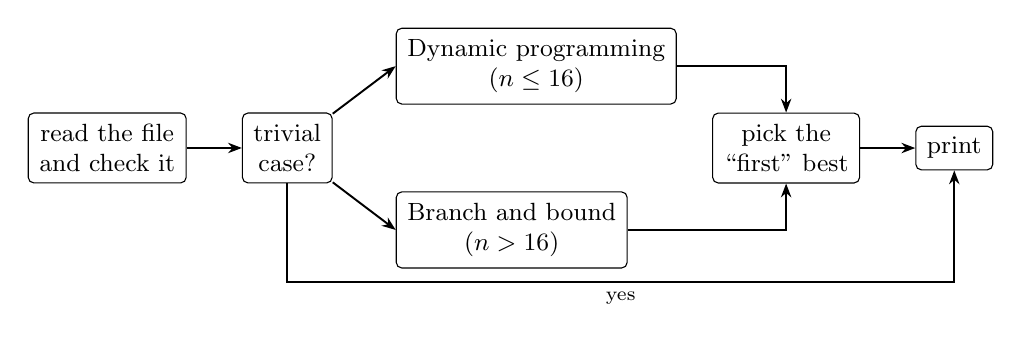
\begin{tikzpicture}[node distance=5mm and 7mm]
  \node[box] (in) {read the file\\and check it};
  \node[box,right=of in] (q) {trivial\\case?};
  \node[box,above right=1mm and 8mm of q] (dp) {Dynamic programming\\($n \le 16$)};
  \node[box,below right=1mm and 8mm of q] (bb) {Branch and bound\\($n > 16$)};
  \node[box] (c) at ($(dp.east)!0.5!(bb.east)+(1.7,0)$) {pick the\\``first'' best};
  \node[box,right=of c] (out) {print};
  \draw[arr] (in)--(q); \draw[arr] (q)--(dp.west); \draw[arr] (q)--(bb.west);
  \draw[arr] (dp.east) -| (c.north); \draw[arr] (bb.east) -| (c.south); \draw[arr] (c)--(out);
  \draw[arr] (q.south) -- ++(0,-1.25) -| node[pos=0.25,below,font=\scriptsize]{yes} (out.south);
\end{tikzpicture}
\caption{Program flow.}
\end{figure}

\subsection{Branch and Bound}

\textbf{Overview.} Color vertices one at a time, backtracking when a vertex
has no legal color, and keep the best coloring found. Exhaustive search is
far too slow, so four pruning rules are added.

\begin{enumerate}
  \item \textbf{Symmetry breaking.} Swapping all Yellows and Blues gives the
        same groups, so a vertex may use only a color already in use or the
        \emph{next} new one. This removes up to $k!$ copies of every coloring.
  \item \textbf{Bounding.} For each group, compute how large it could still
        grow: its current size plus the uncolored vertices with no neighbor
        in it. This limits how small the biggest group and how large the
        smallest group can end up. If even this best case is no better than
        the best found, the branch is pruned (Figure~3).
  \item \textbf{Forward checking.} Once all $k$ groups are opened, if an
        uncolored vertex already has a neighbor in every one of the $k$
        groups, the branch is dead. (Before that, the vertex could still
        open a new group.)
  \item \textbf{Ordering heuristics.} Color the most-connected vertices
        first, since they are the most constrained, and try the smallest
        group first so balanced answers appear early.
\end{enumerate}

\begin{figure}[h]
\centering
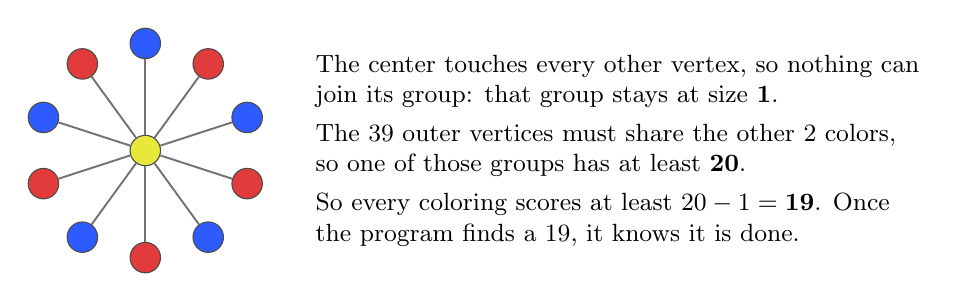
\begin{tikzpicture}[scale=0.85]
  \node[Y] (c) at (0,0) {};
  \foreach \i in {0,...,9} {
    \pgfmathsetmacro{\ang}{90+36*\i}
    \ifodd\i \node[R] (l\i) at (\ang:1.6) {}; \else \node[B] (l\i) at (\ang:1.6) {}; \fi
    \draw[e] (c)--(l\i);
  }
  \node[font=\small,align=left,anchor=west] at (2.4,0)
    {The center touches every other vertex, so nothing can\\
     join its group: that group stays at size \textbf{1}.\\[3pt]
     The 39 outer vertices must share the other 2 colors,\\
     so one of those groups has at least \textbf{20}.\\[3pt]
     So every coloring scores at least $20-1=\mathbf{19}$. Once\\
     the program finds a 19, it knows it is done.};
\end{tikzpicture}
\caption{Bounding on a star with 39 outer vertices and $k=3$. Without it
the program ran for over a minute. With it: 6 milliseconds.}
\end{figure}

\subsection{Dynamic Programming over Subsets}

\textbf{Overview.} Build the coloring \emph{one color group at a time}
instead of one vertex at a time. The subproblem is:

\begin{center}
``Can this set of vertices be split into $j$ groups, with no edge inside
any group and every group size between \emph{lo} and \emph{hi}?''
\end{center}

\begin{minipage}{0.5\textwidth}
\textbf{Recurrence.} Remove a legal group $T$ containing the first vertex of
$S$ (so each split is counted once). If the rest splits into $j-1$ groups,
then $S$ splits into $j$.

\textbf{Overlapping subproblems.} The same subsets recur, so each answer is
stored in a table and computed only once.
\end{minipage}\hfill
\begin{minipage}{0.46\textwidth}
\centering
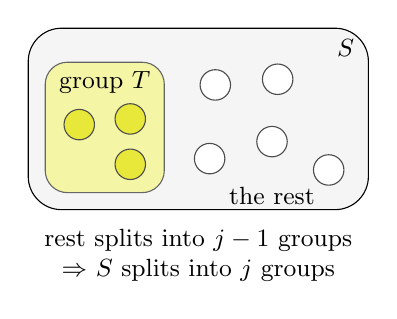
\begin{tikzpicture}[scale=0.72]
  \draw[rounded corners=12pt,fill=black!4] (0,0) rectangle (6,3.2);
  \node[font=\small] at (5.6,2.85) {$S$};
  \draw[rounded corners=8pt,fill=cY!45,draw=black!60] (0.3,0.3) rectangle (2.4,2.6);
  \node[font=\small] at (1.35,2.25) {group $T$};
  \node[Y] at (0.9,1.5) {}; \node[Y] at (1.8,0.8) {}; \node[Y] at (1.8,1.6) {};
  \node[W] at (3.3,2.2) {}; \node[W] at (4.4,2.3) {}; \node[W] at (3.2,0.9) {};
  \node[W] at (4.3,1.2) {}; \node[W] at (5.3,0.7) {};
  \node[font=\small] at (4.3,0.25) {the rest};
  \node[font=\small,align=center] at (3,-0.8)
    {rest splits into $j-1$ groups\\$\Rightarrow$ $S$ splits into $j$ groups};
\end{tikzpicture}
\end{minipage}

\textbf{Optimization.} First check whether \emph{any} $k$-coloring exists.
Then try size ranges from most to least equal (spread 0, then 1, 2,
\dots). The first range that works gives the best score.

\textbf{Example (Figure 1 graph, $k=3$).} Try ``every group has exactly 2
vertices.'' Take a group with vertex 1: $\{1,5\}$ (no edge between them).
The rest is $\{2,3,4,6\}$; take a group with vertex 2: $\{2,6\}$. The rest is
$\{3,4\}$, which is a legal group. That works, so the answer is $(2,2,2)$.

\subsection{Solver Selection}
\begin{tabular}{@{}lll@{}}
\toprule
 & Dynamic programming & Branch and bound \\
\midrule
Time & always about the same (predictable) & usually very fast, but bad cases exist \\
Memory & a table entry for every set of vertices ($2^n$) & very little \\
Used for & 16 vertices or fewer & more than 16 vertices \\
\bottomrule
\end{tabular}

The cutoff of 16 comes from timing tests (Section~\ref{sec:complexity}):
up to 16 vertices, DP's fixed cost stays under 20 milliseconds, so we get
its predictable running time for free. Beyond that its cost grows by
$9\times$ every 2 vertices.

\subsection{Deterministic Output}
A graph often has several best colorings. The program always prints an
optimal one, and it is the ``first'' one unless the search cap in
Section~\ref{sec:complexity} is hit: vertex 1 gets the earliest color it
can, then vertex 2, and so on. Colors are named in order of first use
(Yellow, Blue, Red, Green, \dots, Cyan); after these 12, they are named
``Color 13'', ``Color 14'', and so on. Lines are sorted by group size,
largest first, then by name. This makes the output deterministic and
reproducible.

%=====================================================================
\section{Data Structures}

\textbf{Each set of vertices is one 64-bit integer}, one bit per vertex.
Checking whether vertex $v$ has a neighbor in a group is then a
\emph{single} AND instead of a loop.

\textbf{Limit:} this caps the input at $n = 64$; larger inputs are rejected
with an error. DP is capped at $n \le 20$ by time, not memory: its tables
at $n=20$ take only about 5\,MB ($2^{20}$ entries), but one pass already
takes about $3^{20} \approx 3.5$ billion steps. The program only uses it up
to 16.

\begin{center}
\begin{tabular}{@{}lcccccc@{\qquad}l@{}}
\toprule
vertex & 1 & 2 & 3 & 4 & 5 & 6 & \\
\midrule
neighbors of vertex 3 & 1 & 1 & 0 & 0 & 1 & 1 & \\
group $\{4\}$          & 0 & 0 & 0 & 1 & 0 & 0 & \\
\midrule
AND                    & 0 & 0 & 0 & 0 & 0 & 0 & $\Rightarrow$ no conflict: 3 can join 4's group \\
\bottomrule
\end{tabular}
\end{center}

\noindent\begin{minipage}{\textwidth}
\begin{tabular}{@{}>{\raggedright\arraybackslash}p{4.6cm}>{\raggedright\arraybackslash}p{11cm}@{}}
\toprule
Structure & What it is for \\
\midrule
neighbor sets (one number per vertex) & who is next to whom; conflict checks in one step \\
group sets and group-neighbor sets & who is in each color group, and who touches it; used for conflict checks and for ``how big can this group still get'' \\
DP table ``is this set legal?'' & one entry per set of vertices: true if there is no edge inside it \\
DP table ``how many groups?'' & one number per set; bit $j$ is on if the set splits into $j$ groups, so all values of $j$ are handled at once \\
arrays & each vertex's color, each group's size, the order to color vertices in \\
\bottomrule
\end{tabular}
\end{minipage}

%=====================================================================
\section{Major Functions}

\begin{tabular}{@{}lll@{}}
\toprule
File & Function & What it does \\
\midrule
io.c   & \texttt{read\_input}    & reads $k$, $n$ and the matrix; checks the file is valid \\
       & \texttt{is\_connected}  & checks the graph is in one piece (warns if not) \\
       & \texttt{print\_result}  & prints the group sizes and the vertices in each color \\
dp.c   & \texttt{solve\_dp}      & DP solver: tries size ranges from most to least equal \\
       & (setup in \texttt{solve\_dp}) & builds the ``is this set legal?'' table in $O(2^n)$ \\
       & \texttt{fill}           & fills the DP table for one size range \\
       & \texttt{rebuild}        & reads the groups back out of the table \\
bnb.c  & \texttt{solve\_bnb}     & branch-and-bound solver: sets up and runs the search \\
       & \texttt{search}         & one search step: apply the pruning rules, then try each color \\
       & \texttt{water\_fill}    & the smallest the biggest group can end up (bounding) \\
       & \texttt{canonicalize}   & picks the ``first'' best coloring \\
main.c & \texttt{main}           & handles trivial cases, picks a solver, prints \\
graph.h & \texttt{spread\_lower\_bound} & best possible score: 0 if $k$ divides $n$, else 1 \\
\bottomrule
\end{tabular}

%=====================================================================
\section{Complexity Analysis}\label{sec:complexity}

\subsection{Input Size}

Complexity is measured against the \textbf{input size}: the number of
symbols in the file, not the values of the numbers.

\begin{center}
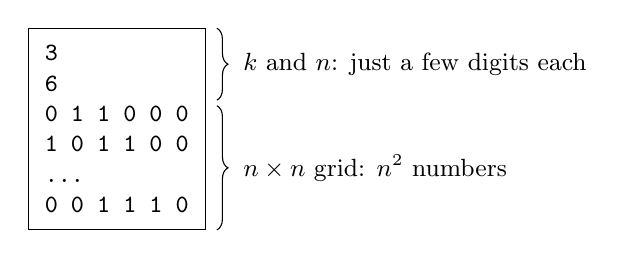
\begin{tikzpicture}
  \node[draw,align=left,font=\ttfamily\small,inner sep=6pt] (f) {3\\6\\0 1 1 0 0 0\\1 0 1 1 0 0\\\dots\\0 0 1 1 1 0};
  \draw[decorate,decoration={brace,amplitude=4pt}] ([xshift=4pt]f.north east) -- ([xshift=4pt,yshift=-26pt]f.north east)
     node[midway,right=6pt,font=\small,align=left] {$k$ and $n$: just a few digits each};
  \draw[decorate,decoration={brace,amplitude=4pt}] ([xshift=4pt,yshift=-28pt]f.north east) -- ([xshift=4pt]f.south east)
     node[midway,right=6pt,font=\small,align=left] {$n \times n$ grid: $n^2$ numbers};
\end{tikzpicture}
\end{center}

\begin{itemize}
  \item $k$ takes about $\log k$ digits, so its \emph{value} does not add to
        the input size.
  \item The $n^2$ grid entries dominate.
  \item If $k>n$ we answer immediately (Section~\ref{sec:problem}), so $k\le n$ from here on.
\end{itemize}
The input size is therefore $N \approx n^2$, so $n = \sqrt{N}$. Each bound
below is given in both $n$ and $N$.

\subsection{Cost by Component}

\begin{itemize}
  \item \textbf{Reading and checking the file.} Each of the $n^2$ entries is
        read and checked once: $O(n^2) = O(N)$, \textbf{linear in the input
        size}.
  \item \textbf{Printing.} Each vertex is printed once and the $k$ lines are
        sorted: $O(n^2)$.
  \item \textbf{Branch and bound.} Each of the $n$ vertices tries at most $k$
        colors, giving $O(k^n)$ nodes in the search tree. Each node computes
        every group's room to grow and does forward checking ($O(k)$ one-word
        bitset operations), runs the bounding binary search ($O(k\log n)$),
        and sorts the candidate colors ($O(k^2)$): $O(k^2 + k\log n)
        \subseteq O(n^2)$ per node. Total: $O(k^n \cdot n^2)$, or
        $O(n^{n+2})$ since $k \le n$. Symmetry breaking visits each \emph{split} into groups only
        once, saving about a factor of $k!$, but $k^n$ remains a simple upper
        bound.
  \item \textbf{Dynamic programming.} A pass visits every set and every group
        inside it. Each vertex is outside the set, in the group, or in the
        rest, so a pass costs about $3^n$. At most about $n^2$ size ranges are
        tried: $O(n^2 \cdot 3^n)$ time and $O(2^n)$ memory.
  \item \textbf{Canonical output.} After a solver finds the best score,
        \texttt{canonicalize} reruns the search in vertex order $1..n$,
        accepting only colorings with that score. It is capped at
        $2\times10^7$ steps; at the cap, the program keeps its existing
        optimal coloring and only renames the colors. This adds a constant
        amount of work, so the totals are unchanged.
\end{itemize}

\subsection{Summary}

\begin{center}
\begin{tabular}{@{}llll@{}}
\toprule
Part & Time in $n$ & Time in input size $N$ & Growth \\
\midrule
Read, check, print & $O(n^2)$ & $O(N)$ & linear \\
Dynamic programming ($n\le16$) & $O(n^2\cdot 3^n)$ & $O(N\cdot 3^{\sqrt N})$ & exponential \\
Branch and bound ($n>16$) & $O(n^{n+2})$ & $2^{O(\sqrt N \log N)}$ & exponential \\
\midrule
Memory: DP & $O(2^n)$ & $O(2^{\sqrt N})$ & exponential \\
Memory: branch and bound & $O(nk)$ & $O(N)$ & small \\
\bottomrule
\end{tabular}
\end{center}

\textbf{Overall.} DP only runs for $n \le 16$, so asymptotically its cost
is a constant. The program's worst case is therefore the branch-and-bound
bound: $O(n^{n+2})$ time, or $2^{O(\sqrt N \log N)}$ in input size.
Branch-and-bound memory is $O(nk)$ because each of the $n$ recursion levels
keeps $O(k)$-sized arrays of group capacities and candidate colors. Group
sets are updated in place and restored on backtrack, not copied.

\textbf{Converting to input size.} Replace $n$ with $\sqrt N$: $3^n$ becomes
$3^{\sqrt N}$, and $n^n = 2^{n\log n}$ becomes $2^{O(\sqrt N \log N)}$.

\textbf{Conclusion.} Reading the input is linear; solving is exponential in
both $n$ and $N$. This is expected, since the problem contains graph
coloring. The pruning rules (Section~\ref{sec:techniques}) make real inputs
fast but do not change the worst case.

\begin{figure}[h]
\centering
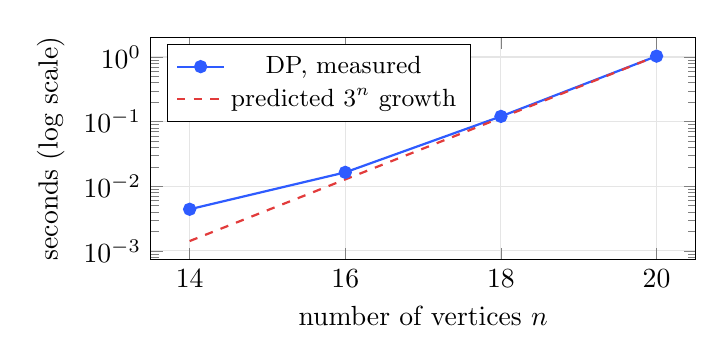
\begin{tikzpicture}
\begin{semilogyaxis}[
  width=8.5cm,height=4.4cm,
  xlabel={number of vertices $n$},ylabel={seconds (log scale)},
  xtick={14,16,18,20},xmin=13.5,xmax=20.5,
  legend style={font=\small,at={(0.03,0.97)},anchor=north west},
  grid=major,grid style={black!10}]
\addplot[mark=*,thick,cB] coordinates {(14,0.0044)(16,0.0164)(18,0.1205)(20,1.0327)};
\addlegendentry{DP, measured}
\addplot[dashed,thick,cR,domain=14:20,samples=7] {1.0327*3^(x-20)};
\addlegendentry{predicted $3^n$ growth}
\end{semilogyaxis}
\end{tikzpicture}
\caption{Measured DP times (random graphs, $k=3$). Each 2 extra vertices
cost about $9\times$ ($3^2$), as predicted. DP already takes 1 second at
20 vertices, so larger graphs use branch and bound, which solved random
graphs of up to 60 vertices in under 0.35 seconds.}
\end{figure}

%=====================================================================
\section{Testing and Validation}

\subsection{Test Suite}

\texttt{make test} runs 1593 checks, and all of them pass.
\begin{itemize}
  \item 38 hand-solved graphs, each run with both solvers, which must agree.
        Every printed coloring is checked: no neighbors share a color, all
        $k$ colors are used, and the sizes match.
  \item A reference sample output must match character for character.
  \item 12 malformed input files must be rejected with an error.
  \item Small random graphs (up to 7 vertices) are checked against brute force.
  \item 150 larger random graphs: DP and branch and bound must agree.
\end{itemize}

\subsection{Worked Examples}

\begin{figure}[h!]
\centering
\newcommand{\tree}[9]{%
\begin{tikzpicture}[scale=0.55]
  \node[#1] (1) at (0,0) {1};    \node[#2] (2) at (0.9,-0.9) {2};
  \node[#3] (3) at (1.8,0.4) {3}; \node[#4] (4) at (2.8,1.3) {4};
  \node[#5] (5) at (4.1,1.3) {5}; \node[#6] (6) at (3.4,0.3) {6};
  \node[#7] (7) at (2.9,-0.6) {7};\node[#8] (8) at (2.4,-1.5) {8};
  \foreach \a/\b in {1/2,2/3,3/4,4/5,3/6,3/7,3/8} \draw[e] (\a)--(\b);
  \node[font=\small] at (2,-2.4) {#9};
\end{tikzpicture}}
\begin{subfigure}[b]{0.3\textwidth}\centering
\tree{Y}{B}{Y}{B}{Y}{B}{B}{B}{$k=2$: $(5,3)$}\\[10pt]
\tree{Y}{B}{Y}{B}{Y}{B}{R}{R}{$k=3$: $(3,3,2)$}
\caption*{An 8-vertex tree}
\end{subfigure}\hfill
\begin{subfigure}[b]{0.66\textwidth}\centering
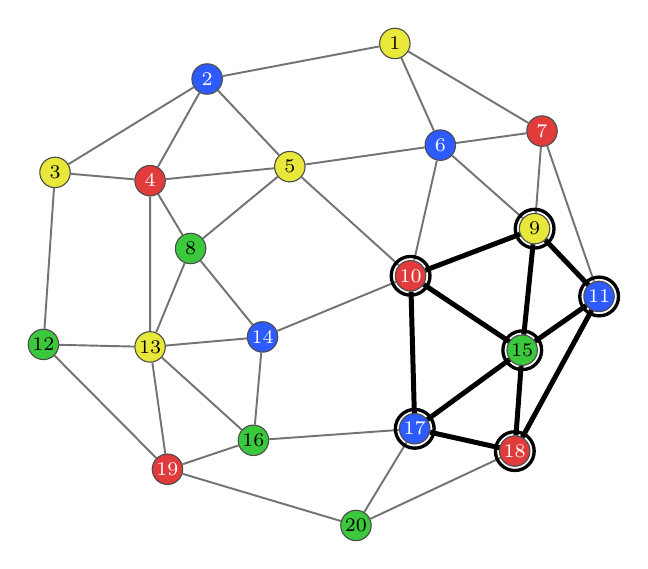
\begin{tikzpicture}[yscale=-1.05,xscale=1.05]
  % vertices A..T = 1..20; colors = program output
  \node[Y] (1) at (5.07,0.47) {1};
  \node[B] (2) at (2.80,0.90) {2};
  \node[Y] (3) at (0.96,2.03) {3};
  \node[R] (4) at (2.11,2.13) {4};
  \node[Y] (5) at (3.80,1.96) {5};
  \node[B] (6) at (5.62,1.70) {6};
  \node[R] (7) at (6.85,1.53) {7};
  \node[G] (8) at (2.60,2.95) {8};
  \node[Y] (9) at (6.76,2.71) {9};
  \node[R] (10) at (5.26,3.28) {10};
  \node[B] (11) at (7.54,3.53) {11};
  \node[G] (12) at (0.82,4.11) {12};
  \node[Y] (13) at (2.11,4.14) {13};
  \node[B] (14) at (3.47,4.02) {14};
  \node[G] (15) at (6.61,4.18) {15};
  \node[G] (16) at (3.36,5.27) {16};
  \node[B] (17) at (5.31,5.13) {17};
  \node[R] (18) at (6.52,5.40) {18};
  \node[R] (19) at (2.32,5.62) {19};
  \node[G] (20) at (4.60,6.30) {20};
  \foreach \a/\b in {1/2,1/6,1/7,2/3,2/4,2/5,3/4,3/12,4/5,4/8,4/13,5/8,5/6,5/10,6/7,6/9,6/10,7/9,7/11,8/13,8/14,10/14,12/13,12/19,13/14,13/16,13/19,14/16,16/17,16/19,17/20,18/20,19/20}
    \draw[e] (\a)--(\b);
  \foreach \a/\b in {9/10,10/17,17/18,18/11,11/9} \draw[hot] (\a)--(\b);
  \foreach \b in {9,10,17,18,11} \draw[hot] (15)--(\b);
  \foreach \n in {9,10,17,18,11,15} \node[draw,circle,line width=1.2pt,minimum size=14pt] at (\n) {};
\end{tikzpicture}
\caption*{A 20-vertex graph: $k=4$ gives $(5,5,5,5)$; $k=3$ gives \textbf{no answer}.}
\end{subfigure}
\caption{Program output on two further examples.}
\end{figure}

\textbf{The 20-vertex graph with $k=3$.} Three colors do not suffice. In the bold part of the right picture, vertex 15 touches every
vertex of the ring 9--10--17--18--11. A ring with an \emph{odd} number of
vertices needs 3 colors (alternating 2 makes the last vertex clash with the
first), so vertex 15 needs a 4th, and the program correctly prints ``no such
a sequence exists.''

\end{document}
